%========================================================================
\documentclass[11pt]{article}
\usepackage{graphics}
\graphicspath{{figs/}}

%===========================================
% Fix the margins
\setlength{\topmargin}{-0.4in}    % distance from top of page to begining of text
\setlength{\textheight}{9.0in}    % height of main text
\setlength{\textwidth}{6.5in}     % width of text
\setlength{\oddsidemargin}{0.in}  % odd page left margin
\setlength{\evensidemargin}{0.in} % even page left margin

%===========================================
\usepackage{amssymb,amsfonts}
\usepackage{amsmath}

%===========================================
\begin{document}

\title{Incompressible Navier Stokes equation using fractional step method}

\author{Zhengjiang Li}

\date{}

\maketitle

\section {Navier-Stokes equation system}

consider incompressible Navier-Stokes equation:

	$$ \frac{\partial u}{\partial t} + ( u \cdot \nabla) u = - \nabla p + \frac{1}{Re} \nabla^2 u $$

	$$ \nabla \cdot u = 0 $$

Straightforwad discretization of these equations will produce a system of equations of the form:
$$ 
\begin{bmatrix} A && G \\ D && 0 \end{bmatrix} \begin{pmatrix} v^{n+1} \\ p^{n+1} \end{pmatrix} = \left( \begin{array}{c} r \\ 0 \end{array} \right) + \left ( \begin{array}{c} bc' \\ bc'' \end{array} \right) $$

discretization with a staggered mesh finite volume formulation, using implicit Crank-Nicolson(CN) integration for the viscous terms and the explicit second-order Adams-Bashforth(AB2) scheme for the convective terms, namely:

\begin{align*}
  \frac{v^{n+1} - v^n}{\Delta t} + [\frac{3}{2} H(v^n) - \frac{1}{2} H(v^{n-1}] \\
 = -G p^{n+1} + \frac{1}{2Re} L(v^{n+1} + v^n) + bc' 
\end{align*}

$$ D v^{n+1} = 0 + bc'' $$

where H operator is the convective operator, G is the gradient operator, L is laplacian operator.

In finite volume method, the primary variables are fluxs and discrete pressure, so the above equation is again written like:
$$ 
\begin{bmatrix} AR^{-1} && G \\ D && 0 \end{bmatrix} \begin{pmatrix} q^{n+1} \\ \phi ^{n+1} \end{pmatrix} = \left( \begin{array}{c} r \\ 0 \end{array} \right) + \left ( \begin{array}{c} bc' \\ bc'' \end{array} \right) $$

where

$$ A = \frac{1}{\Delta t} [ I - \frac{\Delta t}{2Re}L] $$

$$ r_{explicit term} = \frac{1}{\Delta t} [ I + \frac{\Delta t}{2Re} L] v^n - [\frac{3}{2} H(v^n) - \frac{1}{2} H(v^{n-1}] $$

$R$ is the dialogal matrix of x-spacing, y-spacing in each cell.

\section{finite volume algorithm in staggered mesh}

\begin{figure}[!h]
	\caption{p, u, v on staggered mesh}
	\centering
	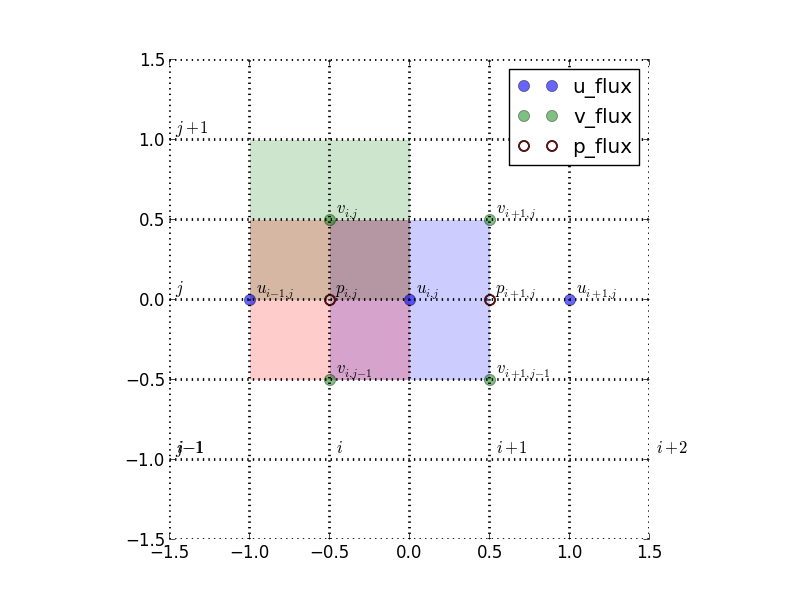
\includegraphics{staggeredmesh}
\end{figure}

e.g. consider x-momentum equation with AB2 for convective term and Crank-Nickson for diffusion term:

$$ \frac{\partial}{\partial t} \int _{\Omega _{ij}} u dV = \int_{\partial \Omega_{ij}} ( -u^2 n_x - u v n_y - p n_x + \nu (u_x n_x + u_y n_y) ) dA  $$

The first term in a grid cell shown in figure above, can be evaluated as

$$  \frac{\partial}{\partial t} \int _{\Omega _{ij}} u dV = \frac{\partial}{\partial t} u_{i,j-1/2} h_x h_y $$

the convective term is defined on cell faces, while the averages must be used, which is then

$$  \int_{\partial \Omega_{ij}} u^2 n_x + u v n_y dA \approx = (\hat{u}_{i+1/2, j-1/2} ^ 2 - \hat{u}_{i-1/2, j-1/2}^2) h_y + ( \hat(v)_{ij} \tilde{u}_{ij} - \hat{v}_{i,j-1} \tilde{u}_{i,j-1}) h_x $$

and viscosity term is

$$ Vis_term = \frac{1}{Re}( \frac{1}{h_x^2} (u_{i+1,j} - 2u_{ij} + u{i-1,j}) + \frac{1}{h_y^2}( u_{i,j+1} - 2u_{i,j} + u_{i,j-1}) ) h_x h_y $$


\section{fractional step method}

For an algebraic system of equation above, usually we can approximate the divergence equation(the second block equation), or we can approximate the momentum equation by approximation the pressure term, as 

 $$ 
\begin{bmatrix} A &&  (AB)G \\ D &&  0 \end{bmatrix} \begin{pmatrix} q^{n+1} \\ \phi ^{n+1} \end{pmatrix} = \left( \begin{array}{c} r_{explicit term} \\ 0 \end{array} \right) + \left ( \begin{array}{c} bc' \\ bc'' \end{array} \right) $$


As discussed in reference paper 1, we can take the block LU decomposition of the Navier-Stokes system above:

$$ 
\begin{bmatrix} A && 0 \\ D && -DBG \end{bmatrix} \begin{pmatrix} q^* \\ \phi ^{n+1} \end{pmatrix} = \left( \begin{array}{c} r \\ 0 \end{array} \right) + \left ( \begin{array}{c} bc' \\ bc'' \end{array} \right) $$

$$ 
\begin{bmatrix} I &&  BG \\ 0 && I \end{bmatrix} \begin{pmatrix} q^{n+1} \\ \phi ^{n+1} \end{pmatrix} = \left( \begin{array}{c} v^* \\ p^{n+1} \end{array} \right) $$

usually, we also call it as projection method, and look like the following:

\begin{align}
	A q^* = r + bc';
	\\ DBG \phi ^{n+1} = D q^* - bc'' ;
  	\\ q^{n+1} = q* - BG \phi ^{n+1};
\end{align}

if B is chosen equal to $\Delta t$ times the identity matrix, then it give the first-order block LU decomposition;
if B is cosen to be an approximate inverse of A, then higher order accuray can be achieved. We will do this approximation here.

\section{Building Matrix and Vectors}

there are 4 matrixs we need to build in this method. Matrix A is a 5-point stencil Laplacian operator minus unit matrix; Matrix Q is centeral difference at half-point, since stagger grid, flux at boundary is store at the middle of surface, so which will bring $[-1, 1]$ stencil, for the off-dialog part of Matrix Q is null space, inserting 0. Matrix B is approximate of inverse A. For $Re>>0$, $A^{-1} \approx \Delta t I$. And the flux-velocity transfer matrix R, is simply the x-spacing,y-spacing of cell.For simple uniform x-spacing, y-spacing is also unit matrix. 



In the final projection system, two right hand side terms consistant with intermediate velocity equation and Poisson equation,respectively. 
\begin{align}
	rhs1 = r_{explicit term} + bc1
\\	rhs2 = Q^T q* - bc2
 \end{align}

$bc1$ is the boundary values for momentum equation. e.g. consider left (-X inlet) boundary, and center difference for laplacian operator.

$$ \frac{u_{i,0}^{n+1}}{\Delta t} - Coef_{implicit} (4u_{i,0} - u_{i+1,0} - u_{i-1,0} - u_{i,1} - u_{i,-1}) = r_{explicit term} $$

$u_{i,-1}$ is derived from the boundary value from inlet velocity boundary, which is the known value, so put it on the right hand side, and called it $bc'$.

similar for $bc2$ in divergence equation, which is the known fluxes at boundary.


\section{Implement in Petsc}

For this 2D recantgular domain, we first define dmda for both pressure and x-flux, y-flux, as $pda, uda, vda$, then create all necessary global vectors. The staggered mesh brings different size for $p, u, v$.

\begin{center}
	\begin{tabular}{|l |l |l |l|}
	\hline
	Variable & Interiour resolution & B.C. included \\ \hline
	P	&  nx, ny & (nx+2), (ny+2) \\ \hline
	U	&  (nx-1), ny & (nx+1), (ny+2) \\ \hline
 	V	&  nx, (ny-1) & (nx+2), (ny+1) \\ 
	\hline
	\end{tabular}
\end{center}
  
where $nx,ny$ are the number of cells in x, y direction, respectively.

Then read in initial values for both flux and pressure, and boundary values for fluxes, after that call LocalToGlobalMapping.

The next step is assemblying the matrixes, and vectors. For late immersed boundary problem, part of matrix related to immersed body will be updated in each time step, so this portion should be called in each timestep.

\section{Results \& Analysis}


\section{petsc src}

\section {Reference}
1 An analysis of the fractional step method, J. B. Perot 1993
\\ 2 Analysis of an exact fractional step method, W. Chang 2002
\\ 3 Lectures in computational fluid dynamics of incompressible flow: mathematics, algorithms and implementations, J. M. McDonough 2007

\end{document}
